\documentclass[oneside,a4paper,10pts,article]{memoir}
\usepackage[utf8]{inputenc}

\usepackage{palatino}
\usepackage{graphicx}
\usepackage{todonotes}
\presetkeys{todonotes}{inline}{}

\usepackage{url}
\usepackage[hidelinks,hyperindex]{hyperref}

\captionnamefont{\bfseries}

\usepackage{tikz}
\usetikzlibrary{positioning,arrows}

\usepackage{listings}
\lstdefinelanguage{JavaScript}{
  keywords={break, case, catch, continue, debugger, default, delete,
    do, else, false, finally, for, function, if, in, instanceof, new,
    null, return, switch, this, throw, true, try, typeof, var, void,
    while, with},
  morecomment=[l]{//},
  morecomment=[s]{/*}{*/},
  morestring=[b]',
  morestring=[b]",
  ndkeywords={class, export, boolean, throw, implements, import, this},
  keywordstyle=\color{blue}\bfseries,
  ndkeywordstyle=\color{darkgray}\bfseries,
  identifierstyle=\color{black},
  commentstyle=\color{purple}\ttfamily,
  stringstyle=\color{red}\ttfamily,
  sensitive=true,
  extendedchars=true,
literate=%
{æ}{{\ae}}1
{å}{{\aa}}1
{ø}{{\o}}1
{Æ}{{\AE}}1
{Å}{{\AA}}1
{Ø}{{\O}}1
}

\lstset{
  basicstyle=\ttfamily\footnotesize,
  keywordstyle=\bfseries,
  captionpos=b,
  language=JavaScript
}

% Remove section numbers
\setsecnumdepth{part}

% Remove page numbers
\renewcommand\thepage{}

\title{Processing intro
  \\ {\normalfont\small\scshape Coding Pirates DIKU }} \date{\today}

\begin{document}
\maketitle

% \chapter{Start}

% \begin{enumerate}
% \item Opret en bruger på \url{http://khanacademy.org}. Brug
% evt. \url{http://da.khanacademy.org} for dansk.
% \item Tryk på ``Subjects'' (``Emner'' på dansk)
% \item Vælg ``Computer programming'' i menuen (``Programmering'' på dansk)
% \item New program / Nyt program
% \end{enumerate}

\chapter{Streg-tegninger}
Tast følgende eksempel ind:
\begin{lstlisting}
    ellipse(200, 200, 150, 150);
    ellipse(135, 125, 75, 75);
    ellipse(260, 130, 75, 75);
\end{lstlisting}
Eller prøv i stedet:
\begin{lstlisting}
    rect(50,100,300,200);
    ellipse(200,200,100,100);
    rect(270,110,70,40);
    rect(70,95,30,5);
\end{lstlisting}
Eller:
\begin{lstlisting}
    triangle(200,150,250,280,150,280);
    ellipse(200,115,70,70);

    line(183,191,146,174);
    line(217,191,254,174);
    line(180, 280, 180, 300);
    line(220, 280, 220, 300);
\end{lstlisting}

\vspace{1cm}
\noindent
Prøv at tegne en bil:

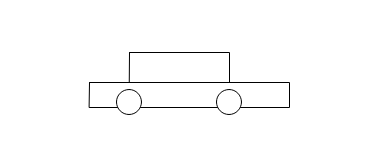
\includegraphics[width=0.7\textwidth]{pics/bil-streg.png}

\newpage
\chapter{Farver}
Farvelæg tegningerne med \texttt{fill}-kommandoen. Det handler om at
sætte \texttt{fill} ind det rigtige sted!
\begin{lstlisting}
  fill(0,0,0);   // sort        fill(0,0,255);     // blå
  fill(255,0,0); // rød         fill(255,255,255); // hvid
  fill(0,255,0); // grøn        fill(0,255,255);   // gul
\end{lstlisting}
\vspace{-3mm}
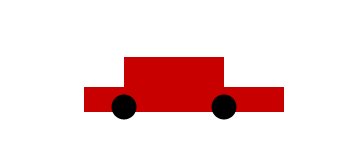
\includegraphics[width=0.5\textwidth]{pics/bil-farvet.png}

\includegraphics[width=0.20\textwidth]{pics/mickey_simpel.png}

\noindent
Prøv også kommandoen:
\begin{lstlisting}
  noStroke();
\end{lstlisting}

\chapter{Opgaver}
\begin{itemize}
\item Kan du tegne en blomst?

  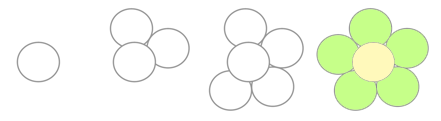
\includegraphics[width=0.5\textwidth]{pics/blomst.png}

\item En pingvin?

  
\includegraphics[width=0.20\textwidth]{pics/pingvin.png}

\item Pikachu?

  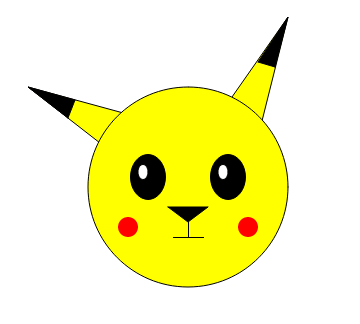
\includegraphics[width=0.3\textwidth]{pics/pikachu.png}
\end{itemize}

\end{document}